% Options for packages loaded elsewhere
\PassOptionsToPackage{unicode}{hyperref}
\PassOptionsToPackage{hyphens}{url}
\documentclass[
]{article}
\usepackage{xcolor}
\usepackage[margin=1in]{geometry}
\usepackage{amsmath,amssymb}
\setcounter{secnumdepth}{-\maxdimen} % remove section numbering
\usepackage{iftex}
\ifPDFTeX
  \usepackage[T1]{fontenc}
  \usepackage[utf8]{inputenc}
  \usepackage{textcomp} % provide euro and other symbols
\else % if luatex or xetex
  \usepackage{unicode-math} % this also loads fontspec
  \defaultfontfeatures{Scale=MatchLowercase}
  \defaultfontfeatures[\rmfamily]{Ligatures=TeX,Scale=1}
\fi
\usepackage{lmodern}
\ifPDFTeX\else
  % xetex/luatex font selection
\fi
% Use upquote if available, for straight quotes in verbatim environments
\IfFileExists{upquote.sty}{\usepackage{upquote}}{}
\IfFileExists{microtype.sty}{% use microtype if available
  \usepackage[]{microtype}
  \UseMicrotypeSet[protrusion]{basicmath} % disable protrusion for tt fonts
}{}
\makeatletter
\@ifundefined{KOMAClassName}{% if non-KOMA class
  \IfFileExists{parskip.sty}{%
    \usepackage{parskip}
  }{% else
    \setlength{\parindent}{0pt}
    \setlength{\parskip}{6pt plus 2pt minus 1pt}}
}{% if KOMA class
  \KOMAoptions{parskip=half}}
\makeatother
\usepackage{color}
\usepackage{fancyvrb}
\newcommand{\VerbBar}{|}
\newcommand{\VERB}{\Verb[commandchars=\\\{\}]}
\DefineVerbatimEnvironment{Highlighting}{Verbatim}{commandchars=\\\{\}}
% Add ',fontsize=\small' for more characters per line
\usepackage{framed}
\definecolor{shadecolor}{RGB}{248,248,248}
\newenvironment{Shaded}{\begin{snugshade}}{\end{snugshade}}
\newcommand{\AlertTok}[1]{\textcolor[rgb]{0.94,0.16,0.16}{#1}}
\newcommand{\AnnotationTok}[1]{\textcolor[rgb]{0.56,0.35,0.01}{\textbf{\textit{#1}}}}
\newcommand{\AttributeTok}[1]{\textcolor[rgb]{0.13,0.29,0.53}{#1}}
\newcommand{\BaseNTok}[1]{\textcolor[rgb]{0.00,0.00,0.81}{#1}}
\newcommand{\BuiltInTok}[1]{#1}
\newcommand{\CharTok}[1]{\textcolor[rgb]{0.31,0.60,0.02}{#1}}
\newcommand{\CommentTok}[1]{\textcolor[rgb]{0.56,0.35,0.01}{\textit{#1}}}
\newcommand{\CommentVarTok}[1]{\textcolor[rgb]{0.56,0.35,0.01}{\textbf{\textit{#1}}}}
\newcommand{\ConstantTok}[1]{\textcolor[rgb]{0.56,0.35,0.01}{#1}}
\newcommand{\ControlFlowTok}[1]{\textcolor[rgb]{0.13,0.29,0.53}{\textbf{#1}}}
\newcommand{\DataTypeTok}[1]{\textcolor[rgb]{0.13,0.29,0.53}{#1}}
\newcommand{\DecValTok}[1]{\textcolor[rgb]{0.00,0.00,0.81}{#1}}
\newcommand{\DocumentationTok}[1]{\textcolor[rgb]{0.56,0.35,0.01}{\textbf{\textit{#1}}}}
\newcommand{\ErrorTok}[1]{\textcolor[rgb]{0.64,0.00,0.00}{\textbf{#1}}}
\newcommand{\ExtensionTok}[1]{#1}
\newcommand{\FloatTok}[1]{\textcolor[rgb]{0.00,0.00,0.81}{#1}}
\newcommand{\FunctionTok}[1]{\textcolor[rgb]{0.13,0.29,0.53}{\textbf{#1}}}
\newcommand{\ImportTok}[1]{#1}
\newcommand{\InformationTok}[1]{\textcolor[rgb]{0.56,0.35,0.01}{\textbf{\textit{#1}}}}
\newcommand{\KeywordTok}[1]{\textcolor[rgb]{0.13,0.29,0.53}{\textbf{#1}}}
\newcommand{\NormalTok}[1]{#1}
\newcommand{\OperatorTok}[1]{\textcolor[rgb]{0.81,0.36,0.00}{\textbf{#1}}}
\newcommand{\OtherTok}[1]{\textcolor[rgb]{0.56,0.35,0.01}{#1}}
\newcommand{\PreprocessorTok}[1]{\textcolor[rgb]{0.56,0.35,0.01}{\textit{#1}}}
\newcommand{\RegionMarkerTok}[1]{#1}
\newcommand{\SpecialCharTok}[1]{\textcolor[rgb]{0.81,0.36,0.00}{\textbf{#1}}}
\newcommand{\SpecialStringTok}[1]{\textcolor[rgb]{0.31,0.60,0.02}{#1}}
\newcommand{\StringTok}[1]{\textcolor[rgb]{0.31,0.60,0.02}{#1}}
\newcommand{\VariableTok}[1]{\textcolor[rgb]{0.00,0.00,0.00}{#1}}
\newcommand{\VerbatimStringTok}[1]{\textcolor[rgb]{0.31,0.60,0.02}{#1}}
\newcommand{\WarningTok}[1]{\textcolor[rgb]{0.56,0.35,0.01}{\textbf{\textit{#1}}}}
\usepackage{graphicx}
\makeatletter
\newsavebox\pandoc@box
\newcommand*\pandocbounded[1]{% scales image to fit in text height/width
  \sbox\pandoc@box{#1}%
  \Gscale@div\@tempa{\textheight}{\dimexpr\ht\pandoc@box+\dp\pandoc@box\relax}%
  \Gscale@div\@tempb{\linewidth}{\wd\pandoc@box}%
  \ifdim\@tempb\p@<\@tempa\p@\let\@tempa\@tempb\fi% select the smaller of both
  \ifdim\@tempa\p@<\p@\scalebox{\@tempa}{\usebox\pandoc@box}%
  \else\usebox{\pandoc@box}%
  \fi%
}
% Set default figure placement to htbp
\def\fps@figure{htbp}
\makeatother
\setlength{\emergencystretch}{3em} % prevent overfull lines
\providecommand{\tightlist}{%
  \setlength{\itemsep}{0pt}\setlength{\parskip}{0pt}}
\usepackage{bookmark}
\IfFileExists{xurl.sty}{\usepackage{xurl}}{} % add URL line breaks if available
\urlstyle{same}
% fallback for those not using the hyperref driver hyperxmp:
\makeatletter
\@ifundefined{xmpquote}{\newcommand{\xmpquote}[1]{#1}}{}
\makeatother
\hypersetup{
  pdftitle={QRM2},
  pdfauthor={Groepje 47},
  hidelinks,
  pdfcreator={LaTeX via pandoc}}

\title{QRM2}
\author{Groepje 47}
\date{2026-09-04}

\begin{document}
\maketitle

\section{Week 1}\label{week-1}

\subsection{1 Dataset}\label{dataset}

Find the dataset ``movies5.tsv'' on Canvas. Describe your data set: How
many observations does it have? How many variables are there? How many
subjects? What consists of a subject? {[}4 points{]}

\begin{Shaded}
\begin{Highlighting}[]
\CommentTok{\# Load the dataset}
\NormalTok{movies }\OtherTok{\textless{}{-}} \FunctionTok{read.delim}\NormalTok{(}\StringTok{"movies5.tsv"}\NormalTok{)}

\FunctionTok{nrow}\NormalTok{(movies)}
\DocumentationTok{\#\# [1] 909}
\FunctionTok{ncol}\NormalTok{(movies)}
\DocumentationTok{\#\# [1] 19}

\FunctionTok{length}\NormalTok{(}\FunctionTok{unique}\NormalTok{(movies}\SpecialCharTok{$}\NormalTok{index))}
\DocumentationTok{\#\# [1] 909}
\end{Highlighting}
\end{Shaded}

\textbf{Your Answer:}

Number of observations: 909 observations (rows).

Number of variables: 19 variables (columns).

Number of subjects: 909 subjects (films).

The dataset contains 909 observations and 19 variables, including the
identifier ``index''. There are 909 subjects, each representing an
individual movie. Each row contains one observation with information
about a movie, such as its title, budget, revenue, and runtime. Since
each movie appears exactly once in the dataset, the number of
observations equals the number of subjects.

\subsection{2 Types of variables}\label{types-of-variables}

Which of the following types of variables are present in your data set?
(i) nominal; (ii) ordinal; (iii) interval; (iv) ratio. If present, name
one example of such a variable present in your data set. {[}4 points{]}

\begin{Shaded}
\begin{Highlighting}[]
\CommentTok{\# Show the variables and their data types}
\FunctionTok{str}\NormalTok{(movies)}
\DocumentationTok{\#\# \textquotesingle{}data.frame\textquotesingle{}:    909 obs. of  19 variables:}
\DocumentationTok{\#\#  $ index              : int  4749 1744 960 1810 2889 1527 3520 2050 3755 1390 ...}
\DocumentationTok{\#\#  $ budget             : num  0.0 3.0e+07 5.0e+07 3.0e+07 1.2e+06 ...}
\DocumentationTok{\#\#  $ keywords           : chr  "love independent film best friend true love irish catholic" "alcohol one{-}night stand bed pregnancy and birth condom" "imaginary friend outcast" "christianity jewry roman empire jesus christ suffering" ...}
\DocumentationTok{\#\#  $ original\_language  : chr  "en" "en" "en" "en" ...}
\DocumentationTok{\#\#  $ title              : chr  "The Brothers McMullen" "Knocked Up" "The Adventures of Sharkboy and Lavagirl" "The Passion of the Christ" ...}
\DocumentationTok{\#\#  $ popularity         : num  1.58 22.53 12.31 38.17 3.58 ...}
\DocumentationTok{\#\#  $ release\_date       : chr  "1995{-}08{-}09" "2007{-}06{-}01" "2005{-}06{-}10" "2004{-}02{-}25" ...}
\DocumentationTok{\#\#  $ revenue            : num  0.00 2.19e+08 6.94e+07 6.12e+08 0.00 ...}
\DocumentationTok{\#\#  $ runtime            : int  98 129 92 127 86 137 112 96 93 92 ...}
\DocumentationTok{\#\#  $ vote\_average       : num  6.3 6.2 4.4 6.9 6.2 6.9 6.2 5.2 5.3 6.2 ...}
\DocumentationTok{\#\#  $ vote\_count         : int  23 1214 269 864 50 113 578 559 26 1428 ...}
\DocumentationTok{\#\#  $ genre              : chr  "Drama" "Drama" "Adventure" "Drama" ...}
\DocumentationTok{\#\#  $ release\_year       : int  1995 2007 2005 2004 2002 1995 2002 2015 2001 2009 ...}
\DocumentationTok{\#\#  $ release\_month      : int  8 6 6 2 5 12 4 9 11 1 ...}
\DocumentationTok{\#\#  $ release\_day        : int  9 1 10 25 24 29 11 3 16 22 ...}
\DocumentationTok{\#\#  $ first\_actor        : chr  "Shari Albert" "Seth Rogen" "Taylor Lautner" "Jim Caviezel" ...}
\DocumentationTok{\#\#  $ first\_actor\_gender : chr  "female" "male" "female" "male" ...}
\DocumentationTok{\#\#  $ director\_first\_name: chr  "Edward" "Judd" "Robert" "Mel" ...}
\DocumentationTok{\#\#  $ director\_gender    : chr  "male" "male" "male" "male" ...}

\FunctionTok{unique}\NormalTok{(movies}\SpecialCharTok{$}\NormalTok{genre)}
\DocumentationTok{\#\#  [1] "Drama"       "Adventure"   "Comedy"      "Thriller"    "Documentary"}
\DocumentationTok{\#\#  [6] "Action"      "Fiction"     "Music"       NA            "Animation"  }
\DocumentationTok{\#\# [11] "Family"      "Horror"      "Romance"     "Western"     "Crime"}

\FunctionTok{sort}\NormalTok{(}\FunctionTok{unique}\NormalTok{(movies}\SpecialCharTok{$}\NormalTok{vote\_average))}
\DocumentationTok{\#\#  [1] 0.0 2.3 2.8 2.9 3.0 3.2 3.3 3.4 3.7 3.8 3.9 4.0 4.1 4.2 4.3 4.4 4.5}
\DocumentationTok{\#\# [18] 4.6 4.7 4.8 4.9 5.0 5.1 5.2 5.3 5.4 5.5 5.6 5.7 5.8 5.9 6.0 6.1 6.2}
\DocumentationTok{\#\# [35] 6.3 6.4 6.5 6.6 6.7 6.8 6.9 7.0 7.1 7.2 7.3 7.4 7.5 7.6 7.7 7.8 7.9}
\DocumentationTok{\#\# [52] 8.0 8.3 9.5}

\FunctionTok{head}\NormalTok{(movies}\SpecialCharTok{$}\NormalTok{release\_year)}
\DocumentationTok{\#\# [1] 1995 2007 2005 2004 2002 1995}
\FunctionTok{head}\NormalTok{(movies}\SpecialCharTok{$}\NormalTok{runtime)}
\DocumentationTok{\#\# [1]  98 129  92 127  86 137}
\end{Highlighting}
\end{Shaded}

\textbf{Your Answer:}

\begin{enumerate}
\def\labelenumi{(\roman{enumi})}
\item
  ``Genre'' is a nominal variable, since categories like Comedy, Drama,
  and Action don't have any natural order.
\item
  The dataset does not include an ordinal variable. We treat
  ``vote\_average'' as an interval variable, which assumes equal
  distances between rating points.
\item
  ``Release\_year'' qualifies as an interval variable. The gap between
  two years always means the same thing---ten years is ten years---yet
  there's no true zero. So, moving from 2000 to 2010 is just as much
  time as 2010 to 2020.
\item
  ``Runtime'' is a ratio variable. Time has a true zero, and we can talk
  about its values in terms of multiples---a 120-minute movie is twice
  as long as a 60-minute one.
\end{enumerate}

\subsection{3 Movie profits and
ratings}\label{movie-profits-and-ratings}

A movie studio wants to know which types of movies give maximal profit.
Perform the following steps to provide the movie studio with an analysis
which corresponds to their request:

\begin{enumerate}
\def\labelenumi{\alph{enumi}.}
\item
  Create the variable profits as the revenue of a movie minus its
  budget. Report its mean, median, maximum, and minimum. {[}2 points{]}
\item
  Which movie has the highest profits in your data set and how much are
  these profits? Which movie has the lowest and how much are its
  profits? If multiple movies have the exact same highest or lowest
  profits, give only one example. {[}2 points{]}
\item
  Create a boxplot of the variable profits. Make sure it has an
  appropriate title, and appropriate titles and labels for the x- and
  y-axis. Give Q1, Q2, Q3, and Q4. What does this tell you about the
  nature of making money in the movies industry? {[}2 points{]}
\item
  Add a new variable to your data set the log of profits. When creating
  this variable, what happens to movies for which profits is zero or
  negative? What then happens when you calculate the mean of log of
  profits? {[}2 points{]}
\item
  For movies that have a profit of zero or less, replace log of profits
  with ``NA''. What is now the mean of log of profits? Create a boxplot
  for log of profits, again with an appropriate title, x- and y-axis
  labels. How does it compare to the boxplot you made under c.)? {[}2
  points{]}
\item
  Create a scatterplot of with the runtime of movies on the x-axis and
  the average vote of movies on the y-axis. What do you conclude from
  the scatterplot? Are movies with a longer runtime considered worse or
  better by the audience, or does the audience not have a preference?
  Why do you think this is the case? {[}2 points{]}
\end{enumerate}

For each step, you should provide first all the code you used to answer
the question and then formulate an answer using full sentences.

\subsubsection{Step a}\label{step-a}

\begin{Shaded}
\begin{Highlighting}[]
\CommentTok{\# Create profits variable}
\NormalTok{movies}\SpecialCharTok{$}\NormalTok{profits }\OtherTok{\textless{}{-}}\NormalTok{ movies}\SpecialCharTok{$}\NormalTok{revenue }\SpecialCharTok{{-}}\NormalTok{ movies}\SpecialCharTok{$}\NormalTok{budget}


\FunctionTok{mean}\NormalTok{(movies}\SpecialCharTok{$}\NormalTok{profits)}
\DocumentationTok{\#\# [1] 56284650}

\FunctionTok{median}\NormalTok{(movies}\SpecialCharTok{$}\NormalTok{profits)}
\DocumentationTok{\#\# [1] 2942221}

\FunctionTok{max}\NormalTok{(movies}\SpecialCharTok{$}\NormalTok{profits)}
\DocumentationTok{\#\# [1] 1082730962}

\FunctionTok{min}\NormalTok{(movies}\SpecialCharTok{$}\NormalTok{profits)}
\DocumentationTok{\#\# [1] {-}98301101}
\end{Highlighting}
\end{Shaded}

\textbf{Your Answer:}

We calculated profit by subtracting the budget from the revenue. The
mean profit is 56,284,649.70, and the median is 2,942,221. The highest
profit is 1,082,730,962, and the lowest is −98,301,101.

\subsubsection{Step b}\label{step-b}

\begin{Shaded}
\begin{Highlighting}[]
\CommentTok{\# Movie with the highest profit and its profit}
\NormalTok{movies}\SpecialCharTok{$}\NormalTok{title[}\FunctionTok{which.max}\NormalTok{(movies}\SpecialCharTok{$}\NormalTok{profits)]}
\DocumentationTok{\#\# [1] "Minions"}
\FunctionTok{max}\NormalTok{(movies}\SpecialCharTok{$}\NormalTok{profits)}
\DocumentationTok{\#\# [1] 1082730962}

\NormalTok{movies}\SpecialCharTok{$}\NormalTok{title[}\FunctionTok{which.min}\NormalTok{(movies}\SpecialCharTok{$}\NormalTok{profits)]}
\DocumentationTok{\#\# [1] "The 13th Warrior"}
\FunctionTok{min}\NormalTok{(movies}\SpecialCharTok{$}\NormalTok{profits)}
\DocumentationTok{\#\# [1] {-}98301101}
\end{Highlighting}
\end{Shaded}

\textbf{Your Answer:}

``Minions'' has the highest profit, earning 1,082,730,962 above its
budget. ``The 13th Warrior'' has the lowest profit, with a loss of
98,301,101. This result was also found with max/min in step a.

\subsubsection{Step c}\label{step-c}

\begin{Shaded}
\begin{Highlighting}[]
\CommentTok{\# Boxplot of profits in millions}
\FunctionTok{boxplot}\NormalTok{(movies}\SpecialCharTok{$}\NormalTok{profits }\SpecialCharTok{/} \DecValTok{1000000}\NormalTok{,}
        \AttributeTok{main =} \StringTok{"Movie profits"}\NormalTok{,}
        \AttributeTok{xlab =} \StringTok{"All movies"}\NormalTok{,}
        \AttributeTok{ylab =} \StringTok{"Profit (millions)"}\NormalTok{,}
        \AttributeTok{col =} \StringTok{"lightblue"}\NormalTok{)}
\end{Highlighting}
\end{Shaded}

\pandocbounded{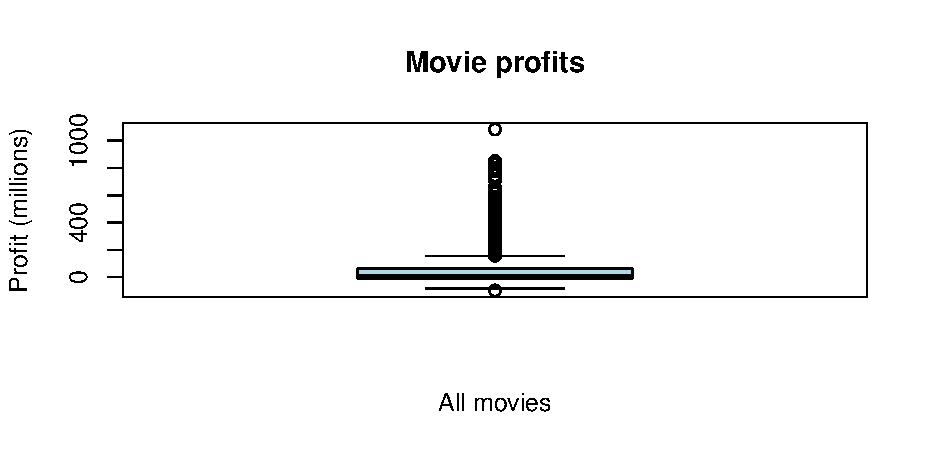
\includegraphics[keepaspectratio]{Untitled_files/Untitled_files/figure-latex/unnamed-chunk-5-1.pdf}}

\begin{Shaded}
\begin{Highlighting}[]

\FunctionTok{summary}\NormalTok{(movies}\SpecialCharTok{$}\NormalTok{profits)}
\DocumentationTok{\#\#       Min.    1st Qu.     Median       Mean    3rd Qu.       Max. }
\DocumentationTok{\#\#  {-}98301101   {-}1260859    2942221   56284650   61340801 1082730962}
\end{Highlighting}
\end{Shaded}

\textbf{Your Answer:}

Q1 is −1,260,859, Q2 is 2,942,221, and Q3 is 61,340,801. We interpret Q4
as the maximum, which is 1,082,730,962.

The boxplot shows that a few movies make much higher profits than the
rest, which pulls the mean above the median. Based on the recorded
revenue and budget, at least a quarter of the movies made a loss. This
suggests that making movies can be risky: some earn huge profits, while
many others earn much less or lose money.

\subsubsection{Step d}\label{step-d}

\begin{Shaded}
\begin{Highlighting}[]
\CommentTok{\# Create the natural logarithm of profits}
\NormalTok{movies}\SpecialCharTok{$}\NormalTok{log\_profits }\OtherTok{\textless{}{-}} \FunctionTok{log}\NormalTok{(movies}\SpecialCharTok{$}\NormalTok{profits)}
\DocumentationTok{\#\# Warning in log(movies$profits): NaNs produced}

\CommentTok{\# Count movies with zero or negative profits}
\FunctionTok{sum}\NormalTok{(movies}\SpecialCharTok{$}\NormalTok{profits }\SpecialCharTok{==} \DecValTok{0}\NormalTok{)}
\DocumentationTok{\#\# [1] 162}
\FunctionTok{sum}\NormalTok{(movies}\SpecialCharTok{$}\NormalTok{profits }\SpecialCharTok{\textless{}} \DecValTok{0}\NormalTok{)}
\DocumentationTok{\#\# [1] 261}

\FunctionTok{mean}\NormalTok{(movies}\SpecialCharTok{$}\NormalTok{log\_profits)}
\DocumentationTok{\#\# [1] NaN}
\end{Highlighting}
\end{Shaded}

\textbf{Your Answer:}

For movies with zero profit, taking the logarithm gives −Inf. For movies
with negative profit, it gives NaN, and R shows a warning. There are 162
movies with zero profit and 261 with negative profit. Because the
log-profit variable contains these values, it means the calculation of
the mean becomes NaN. You would have to filter out these NaN and -Inf to
correctly calculate the mean of movies with more than 0 profit.

\subsubsection{Step e}\label{step-e}

\begin{Shaded}
\begin{Highlighting}[]
\CommentTok{\# Replace log profits with NA for non{-}positive profits}
\NormalTok{movies}\SpecialCharTok{$}\NormalTok{log\_profits[movies}\SpecialCharTok{$}\NormalTok{profits }\SpecialCharTok{\textless{}=} \DecValTok{0}\NormalTok{] }\OtherTok{\textless{}{-}} \ConstantTok{NA}

\FunctionTok{mean}\NormalTok{(movies}\SpecialCharTok{$}\NormalTok{log\_profits, }\AttributeTok{na.rm =} \ConstantTok{TRUE}\NormalTok{)}
\DocumentationTok{\#\# [1] 17.5448}

\FunctionTok{boxplot}\NormalTok{(}
\NormalTok{  movies}\SpecialCharTok{$}\NormalTok{log\_profits,}
  \AttributeTok{main =} \StringTok{"Distribution of Log Movie Profits"}\NormalTok{,}
  \AttributeTok{xlab =} \StringTok{"Movies"}\NormalTok{,}
  \AttributeTok{ylab =} \StringTok{"Natural logarithm of profit"}\NormalTok{,}
  \AttributeTok{names =} \StringTok{"Positive{-}profit movies"}\NormalTok{,}
  \AttributeTok{col =} \StringTok{"lightgreen"}
\NormalTok{)}
\end{Highlighting}
\end{Shaded}

\pandocbounded{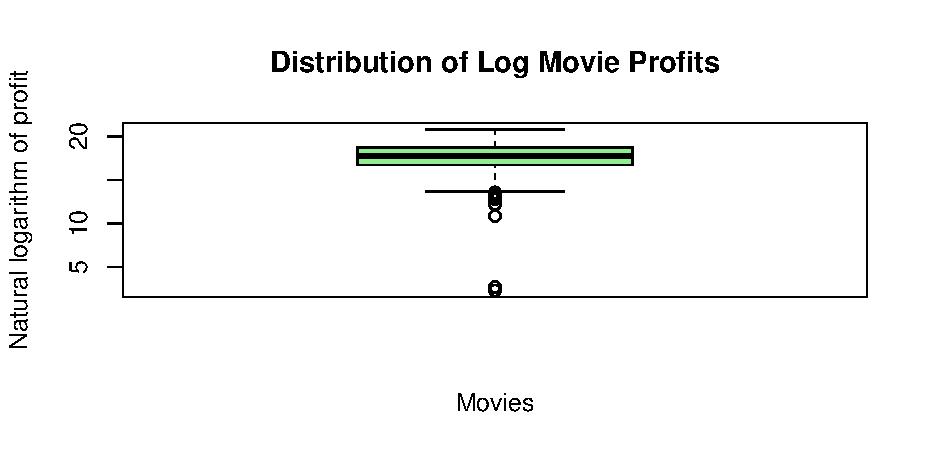
\includegraphics[keepaspectratio]{Untitled_files/Untitled_files/figure-latex/unnamed-chunk-7-1.pdf}}

\textbf{Your Answer:}

After replacing the log values for zero and negative profits with NA,
the mean log profit is about 17.5448. We used na.rm = TRUE to leave out
the missing values, so this mean only includes the 486 movies with
positive profits.

The new boxplot is less stretched towards high values because the
logarithm brings large profits closer together. There are still several
outliers on the lower side. The plots also include different movies: the
first includes all movies, while the second only includes movies that
made a positive profit.

\subsubsection{Step f}\label{step-f}

\begin{Shaded}
\begin{Highlighting}[]
\CommentTok{\# Create a scatterplot of runtime and average rating}
\FunctionTok{plot}\NormalTok{(}
\NormalTok{  movies}\SpecialCharTok{$}\NormalTok{runtime,}
\NormalTok{  movies}\SpecialCharTok{$}\NormalTok{vote\_average,}
  \AttributeTok{main =} \StringTok{"Movie Runtime and Average Audience Rating"}\NormalTok{,}
  \AttributeTok{xlab =} \StringTok{"Runtime (minutes)"}\NormalTok{,}
  \AttributeTok{ylab =} \StringTok{"Average audience rating"}\NormalTok{,}
  \AttributeTok{pch =} \DecValTok{19}\NormalTok{,}
  \AttributeTok{col =} \FunctionTok{rgb}\NormalTok{(}\DecValTok{0}\NormalTok{, }\FloatTok{0.3}\NormalTok{, }\FloatTok{0.7}\NormalTok{, }\FloatTok{0.4}\NormalTok{)}
\NormalTok{)}
\end{Highlighting}
\end{Shaded}

\pandocbounded{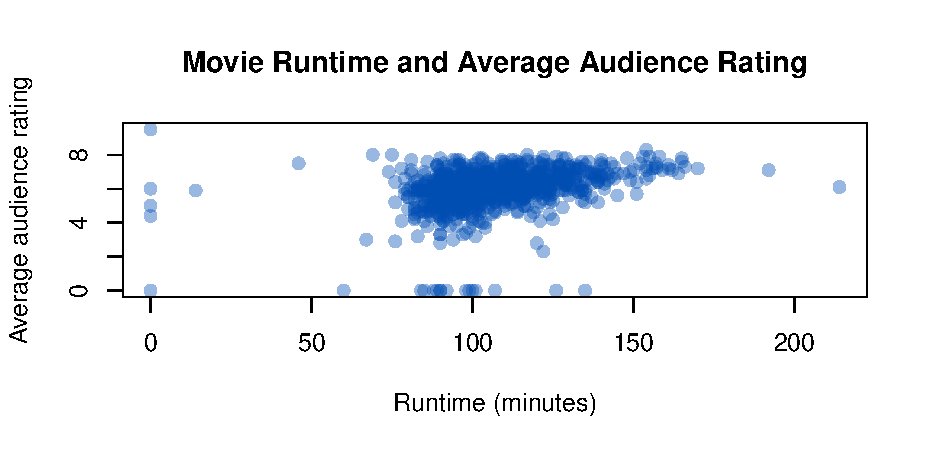
\includegraphics[keepaspectratio]{Untitled_files/Untitled_files/figure-latex/unnamed-chunk-8-1.pdf}}

\begin{Shaded}
\begin{Highlighting}[]

\FunctionTok{cor}\NormalTok{(movies}\SpecialCharTok{$}\NormalTok{runtime, movies}\SpecialCharTok{$}\NormalTok{vote\_average)}
\DocumentationTok{\#\# [1] 0.3204062}
\end{Highlighting}
\end{Shaded}

\textbf{Your Answer:}

The scatterplot suggests that longer movies tend to receive slightly
higher ratings. The correlation is about 0.32, but the points are spread
out, so there are plenty of exceptions.

Longer movies might have more time to develop their characters and
stories, which could help explain the higher ratings. Genre and movie
quality could also play a role. The plot does not prove that making a
movie longer will improve its rating. There are also some zero values
for runtime and rating that may represent missing or incorrectly
recorded data. These values should be investigated before drawing firm
conclusions.

\newpage

\section{Week 2}\label{week-2}

\subsection{1 Population and sample}\label{population-and-sample}

Is your dataset movies5.tsv the full population, or is it a sample of a
larger population? If the latter, how would you describe the full
population? {[}4 points{]}

\textbf{Your Answer:}

The dataset is a sample of a larger population because it contains 909
movies, rather than every movie. The full population would be all movies
we want to draw conclusions about. For example, if we want to study
movies released between 1990 and 2016, the population would include all
movies released during those years. We cannot assume that the movies in
our dataset were selected randomly.

\subsection{2 Actors and movie revenue}\label{actors-and-movie-revenue}

\subsubsection{Step a}\label{step-a-1}

For which actor in your data set do you observe the most movies? {[}2
points{]}

\begin{Shaded}
\begin{Highlighting}[]
\CommentTok{\# Count the movies for each actor}
\NormalTok{actor\_counts }\OtherTok{\textless{}{-}} \FunctionTok{table}\NormalTok{(movies}\SpecialCharTok{$}\NormalTok{first\_actor)}

\FunctionTok{head}\NormalTok{(}\FunctionTok{sort}\NormalTok{(actor\_counts, }\AttributeTok{decreasing =} \ConstantTok{TRUE}\NormalTok{))}
\DocumentationTok{\#\# }
\DocumentationTok{\#\#   Bruce Willis      Tom Hanks    Johnny Depp Sandra Bullock     Tom Cruise }
\DocumentationTok{\#\#              8              8              7              7              7 }
\DocumentationTok{\#\# Drew Barrymore }
\DocumentationTok{\#\#              6}
\end{Highlighting}
\end{Shaded}

\textbf{Your Answer:}

Bruce Willis and Tom Hanks appear most often, with 8 movies each. We use
Bruce Willis for the next steps. These counts are based on the
first\_actor column, so they do not include appearances by actors
elsewhere in a movie's cast.

\subsubsection{Step b}\label{step-b-1}

What is the average revenue of the movie in which this actor plays and
does the revenue lie above or below the revenue of an average movie
according to your data set? {[}2 points{]}

\begin{Shaded}
\begin{Highlighting}[]
\CommentTok{\# Average revenue of movies with Bruce Willis as first\_actor}
\FunctionTok{mean}\NormalTok{(movies}\SpecialCharTok{$}\NormalTok{revenue[movies}\SpecialCharTok{$}\NormalTok{first\_actor }\SpecialCharTok{==} \StringTok{"Bruce Willis"}\NormalTok{],}
     \AttributeTok{na.rm =} \ConstantTok{TRUE}\NormalTok{)}
\DocumentationTok{\#\# [1] 228062987}

\FunctionTok{mean}\NormalTok{(movies}\SpecialCharTok{$}\NormalTok{revenue, }\AttributeTok{na.rm =} \ConstantTok{TRUE}\NormalTok{)}
\DocumentationTok{\#\# [1] 88846315}
\end{Highlighting}
\end{Shaded}

\textbf{Your Answer:}

The average revenue of the movies with Bruce Willis is 228,062,987.38.
The average revenue across all movies in the dataset is 88,846,314.90.
His movies therefore earn more revenue on average than the average movie
in this dataset.

\subsubsection{Step c}\label{step-c-1}

How trustworthy do you consider your conclusion to answer 2b? Use the
term ``law of large numbers'' in your explanation. {[}2 points{]}

\begin{Shaded}
\begin{Highlighting}[]
\CommentTok{\# Number of movies used for the Bruce Willis average}
\FunctionTok{sum}\NormalTok{(movies}\SpecialCharTok{$}\NormalTok{first\_actor }\SpecialCharTok{==} \StringTok{"Bruce Willis"}\NormalTok{, }\AttributeTok{na.rm =} \ConstantTok{TRUE}\NormalTok{)}
\DocumentationTok{\#\# [1] 8}
\end{Highlighting}
\end{Shaded}

\textbf{Your Answer:}

The comparison is correct for this dataset, but it is based on only 8
Bruce Willis movies. One or two very successful movies could have a
large effect on his average.

The law of large numbers tells us that, with a sufficiently large random
sample, the sample mean tends to get closer to the population mean.
Since we only have 8 movies and do not know whether they were randomly
selected, we should be careful about applying this result to all Bruce
Willis movies. It also does not show that Bruce Willis himself causes
higher revenue.

\subsection{3 Population and sample
variance}\label{population-and-sample-variance}

For this question, you will assume that your data set is the full
population.

\subsubsection{Step a}\label{step-a-2}

Recode profits such that it is expressed in millions. What is the
variance of the variable profits (in millions) in your data set? {[}2
points{]}

\begin{Shaded}
\begin{Highlighting}[]
\CommentTok{\# Calculate profits in millions}
\NormalTok{movies}\SpecialCharTok{$}\NormalTok{profits }\OtherTok{\textless{}{-}}\NormalTok{ (movies}\SpecialCharTok{$}\NormalTok{revenue }\SpecialCharTok{{-}}\NormalTok{ movies}\SpecialCharTok{$}\NormalTok{budget) }\SpecialCharTok{/} \DecValTok{1000000}

\CommentTok{\# Calculate the population variance}
\NormalTok{population\_variance }\OtherTok{\textless{}{-}} \FunctionTok{mean}\NormalTok{(}
\NormalTok{  (movies}\SpecialCharTok{$}\NormalTok{profits }\SpecialCharTok{{-}} \FunctionTok{mean}\NormalTok{(movies}\SpecialCharTok{$}\NormalTok{profits))}\SpecialCharTok{\^{}}\DecValTok{2}
\NormalTok{)}

\NormalTok{population\_variance}
\DocumentationTok{\#\# [1] 17802.62}
\end{Highlighting}
\end{Shaded}

\textbf{Your Answer:}

The population variance of profits is approximately 17,802.62 squared
million dollars. The variance is calculated using squared deviations
from the mean, so negative and positive deviations do not cancel each
other out. We divide by N, rather than N−1, because the assignment asks
us to treat the dataset as the full population.

\subsubsection{Step b}\label{step-b-2}

Create a new data set, called movies\_sample. Make sure that it is a
random sample of your data set of 25 movies. What is the variance of
profits in this random sample? How does it compare to the variance of
profits in 2a? {[}2 points{]}

\begin{Shaded}
\begin{Highlighting}[]
\CommentTok{\# Make the random sample reproducible}
\FunctionTok{set.seed}\NormalTok{(}\DecValTok{47}\NormalTok{)}

\NormalTok{movies\_sample }\OtherTok{\textless{}{-}}\NormalTok{ movies[}\FunctionTok{sample}\NormalTok{(}\FunctionTok{nrow}\NormalTok{(movies), }\DecValTok{25}\NormalTok{), ]}

\FunctionTok{var}\NormalTok{(movies\_sample}\SpecialCharTok{$}\NormalTok{profits)}
\DocumentationTok{\#\# [1] 15728.93}
\end{Highlighting}
\end{Shaded}

\textbf{Your Answer:}

The sample variance is approximately 15,728.93 squared millions. This is
lower than the population variance of 17,802.62 from the previous step.

The values differ because the sample contains only 25 of the 909 movies.
A different sample could give a higher or lower variance, depending on
which movies are selected.

\subsubsection{Step c}\label{step-c-2}

In a for loop, create 100 different samples of 25 movies, as in b, and
estimate the variance within each sample. Save the variance of each
sample in a vector called sample\_vars. So the first position of the
vector would have the variance of the first sample, the second position
the variance of the second sample, etc. Print the start of this vector.
{[}2 points{]}

\begin{Shaded}
\begin{Highlighting}[]
\CommentTok{\# Make the random samples reproducible}
\FunctionTok{set.seed}\NormalTok{(}\DecValTok{47}\NormalTok{)}

\NormalTok{sample\_vars }\OtherTok{\textless{}{-}} \FunctionTok{numeric}\NormalTok{(}\DecValTok{100}\NormalTok{)}

\CommentTok{\# Take 100 samples and save their variances}
\ControlFlowTok{for}\NormalTok{ (i }\ControlFlowTok{in} \DecValTok{1}\SpecialCharTok{:}\DecValTok{100}\NormalTok{) \{}
\NormalTok{  movies\_sample }\OtherTok{\textless{}{-}}\NormalTok{ movies[}\FunctionTok{sample}\NormalTok{(}\FunctionTok{nrow}\NormalTok{(movies), }\DecValTok{25}\NormalTok{), ]}
\NormalTok{  sample\_vars[i] }\OtherTok{\textless{}{-}} \FunctionTok{var}\NormalTok{(movies\_sample}\SpecialCharTok{$}\NormalTok{profits)}
\NormalTok{\}}

\FunctionTok{head}\NormalTok{(sample\_vars)}
\DocumentationTok{\#\# [1] 15728.93 31971.87 16532.82 28257.89 24848.85 56289.00}
\end{Highlighting}
\end{Shaded}

\textbf{Your Answer:}

We took 100 random samples of 25 movies and saved each sample variance
in sample\_vars. The first six variances are approximately 15,728.93,
31,971.87, 16,532.82, 28,257.89, 24,848.85, and 56,289.00.

The variances differ because each sample contains a different selection
of movies, as explained in step 3b.

\subsubsection{Step d}\label{step-d-1}

Summarize and make a histogram of sample\_vars. What is the mean,
standard deviation and shape of its distribution? {[}2 points{]}

\begin{Shaded}
\begin{Highlighting}[]
\CommentTok{\# Summarize the sample variances}
\FunctionTok{summary}\NormalTok{(sample\_vars)}
\end{Highlighting}
\end{Shaded}

\begin{verbatim}
##    Min. 1st Qu.  Median    Mean 3rd Qu.    Max. 
##   875.3  6303.8 16465.8 19982.6 26872.9 80456.9
\end{verbatim}

\begin{Shaded}
\begin{Highlighting}[]
\FunctionTok{mean}\NormalTok{(sample\_vars)}
\end{Highlighting}
\end{Shaded}

\begin{verbatim}
## [1] 19982.63
\end{verbatim}

\begin{Shaded}
\begin{Highlighting}[]
\FunctionTok{sd}\NormalTok{(sample\_vars)}
\end{Highlighting}
\end{Shaded}

\begin{verbatim}
## [1] 16853.97
\end{verbatim}

\begin{Shaded}
\begin{Highlighting}[]
\FunctionTok{hist}\NormalTok{(sample\_vars,}
     \AttributeTok{main =} \StringTok{"Sample variances of movie profits"}\NormalTok{,}
     \AttributeTok{xlab =} \StringTok{"Sample variance (squared millions)"}\NormalTok{,}
     \AttributeTok{ylab =} \StringTok{"Frequency"}\NormalTok{,}
     \AttributeTok{col =} \StringTok{"lightblue"}\NormalTok{)}
\end{Highlighting}
\end{Shaded}

\pandocbounded{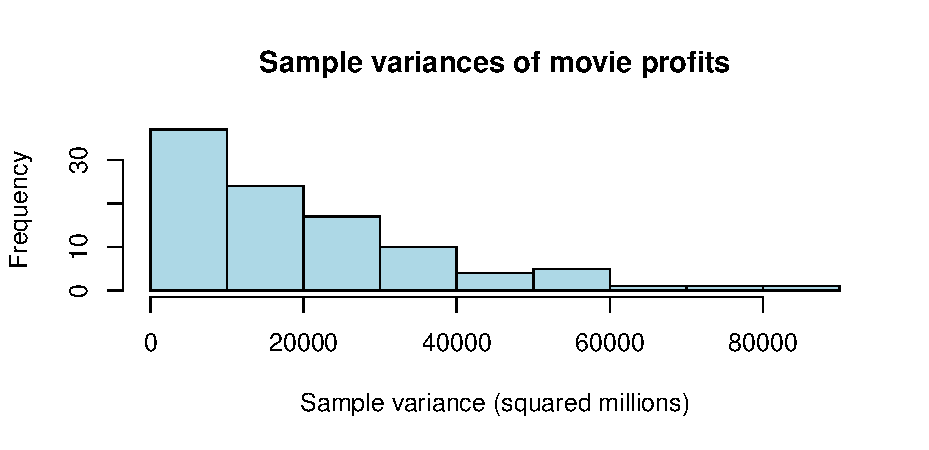
\includegraphics[keepaspectratio]{Untitled_files/Untitled_files/figure-latex/unnamed-chunk-15-1.pdf}}

\textbf{Your Answer:}

The mean of the 100 sample variances is approximately 19,982.63, and the
standard deviation is approximately 16,853.97. Both are expressed in
squared millions.

The histogram shows many lower sample variances and a smaller number of
much higher values, creating a long tail to the right. Samples that
include movies with exceptionally high profits can have much larger
variances than samples without those movies, because their profits are
far above the sample mean. These large differences are squared, giving
them a strong effect on the result.

\subsubsection{Step e}\label{step-e-1}

In your opinion, is a sample of 25 movies sufficient to get a reliable
estimate of the population variance of profits, using the sample
variance? Explain. {[}2 points{]}

\textbf{Your Answer:}

A sample of 25 movies does not seem large enough to give a reliable
estimate of the population variance in this dataset. The sample
variances differ a lot, and their standard deviation is large compared
with their mean.

A few movies have exceptionally high profits. Including or missing one
of these movies can strongly change the sample variance. A larger random
sample would generally give a more stable estimate of the population
variance, in this dataset.

\newpage

\section{Week 3}\label{week-3}

For the next part of the assignment, assume that the movies in your data
frame are a random sample of a larger population of movies.

\subsection{1 Confidence intervals for
runtime}\label{confidence-intervals-for-runtime}

\subsubsection{Step a}\label{step-a-3}

Create a new data set that only includes movies that are of the genre
``Thriller''. For these thriller movies, give a 99 percent confidence
interval for the variable runtime. Interpret the result. {[}2 points{]}

\begin{Shaded}
\begin{Highlighting}[]
\CommentTok{\# Create a dataset with only thriller movies}
\NormalTok{movies\_thriller }\OtherTok{\textless{}{-}} \FunctionTok{subset}\NormalTok{(movies, genre }\SpecialCharTok{==} \StringTok{"Thriller"}\NormalTok{)}

\NormalTok{n\_thriller }\OtherTok{\textless{}{-}} \FunctionTok{nrow}\NormalTok{(movies\_thriller)}
\NormalTok{mean\_runtime }\OtherTok{\textless{}{-}} \FunctionTok{mean}\NormalTok{(movies\_thriller}\SpecialCharTok{$}\NormalTok{runtime)}
\NormalTok{n\_thriller}
\DocumentationTok{\#\# [1] 127}
\NormalTok{mean\_runtime}
\DocumentationTok{\#\# [1] 106.1969}

\CommentTok{\# Calculate the 99\% confidence interval for the mean runtime}
\NormalTok{test\_runtime }\OtherTok{\textless{}{-}} \FunctionTok{t.test}\NormalTok{(movies\_thriller}\SpecialCharTok{$}\NormalTok{runtime, }\AttributeTok{conf.level =} \FloatTok{0.99}\NormalTok{)}
\NormalTok{test\_runtime}\SpecialCharTok{$}\NormalTok{conf.int}
\DocumentationTok{\#\# [1] 102.6930 109.7007}
\DocumentationTok{\#\# attr(,"conf.level")}
\DocumentationTok{\#\# [1] 0.99}
\end{Highlighting}
\end{Shaded}

\textbf{Your Answer:}

There are 127 thriller movies in total, with an average runtime of
approximately 106.20 minutes. The 99\% confidence interval for the
population mean runtime is from 102.69 to 109.70 minutes.

We are 99\% confident that the mean runtime of thriller movies in the
population lies within this interval. This interval is about the
population mean, rather than the runtime of an individual movie. We use
a t-distribution because the population variance is unknown in this
question.

\subsubsection{Step b}\label{step-b-3}

Now, assume that the variance of runtime amongst thriller movies in your
data is exactly the same as the variance of runtime in the population.
Under this assumption, give a 99 percent confidence interval for the
variable runtime among thriller movies. Interpret the result. Is your
confidence interval wider or less wide than the one you found under
question 1a? Why is that the case? {[}2 points{]}

\begin{Shaded}
\begin{Highlighting}[]
\CommentTok{\# Use the sample variance as the known population variance}
\NormalTok{population\_variance\_runtime }\OtherTok{\textless{}{-}} \FunctionTok{var}\NormalTok{(movies\_thriller}\SpecialCharTok{$}\NormalTok{runtime)}

\NormalTok{standard\_error\_runtime }\OtherTok{\textless{}{-}} \FunctionTok{sqrt}\NormalTok{(population\_variance\_runtime }\SpecialCharTok{/}\NormalTok{ n\_thriller)}

\CommentTok{\# Critical z{-}value for a 99\% confidence interval}
\NormalTok{z\_value }\OtherTok{\textless{}{-}} \FloatTok{2.576}

\NormalTok{lower\_runtime }\OtherTok{\textless{}{-}}\NormalTok{ mean\_runtime }\SpecialCharTok{{-}}\NormalTok{ z\_value }\SpecialCharTok{*}\NormalTok{ standard\_error\_runtime}
\NormalTok{upper\_runtime }\OtherTok{\textless{}{-}}\NormalTok{ mean\_runtime }\SpecialCharTok{+}\NormalTok{ z\_value }\SpecialCharTok{*}\NormalTok{ standard\_error\_runtime}

\FunctionTok{c}\NormalTok{(lower\_runtime, upper\_runtime)}
\DocumentationTok{\#\# [1] 102.7458 109.6479}
\end{Highlighting}
\end{Shaded}

\textbf{Your Answer:}

Under this assumption, the 99\% confidence interval is from 102.75 to
109.65 minutes. This means that we are 99\% confident that the true mean
runtime of all thriller movies lies between those two values.

This interval is a little bit narrower than the interval in step a. In
this question, we assume that the population variance is known, so we
use the normal distribution instead of the t-distribution as we did
earlier. For a 99\% confidence interval, we get a critical z-value of
2.576. Because this value is slightly smaller than the t-value used in
the previous step, the confidence interval is also slightly narrower.

\subsection{2 Testing the variance of
runtime}\label{testing-the-variance-of-runtime}

\subsubsection{Step a}\label{step-a-4}

Using an appropriate five-step procedure, set up a test for the null
hypothesis that the variance of runtime equals 500. Clearly state your
null hypothesis, alternative hypothesis, your test statistic, your
critical value, and your conclusion. {[}2 points{]}

\begin{Shaded}
\begin{Highlighting}[]
\CommentTok{\# Number of movies}
\NormalTok{n }\OtherTok{\textless{}{-}} \FunctionTok{nrow}\NormalTok{(movies)}

\NormalTok{sample\_variance }\OtherTok{\textless{}{-}} \FunctionTok{var}\NormalTok{(movies}\SpecialCharTok{$}\NormalTok{runtime)}

\CommentTok{\# Calculate the chi{-}square test statistic}
\NormalTok{chi\_square }\OtherTok{\textless{}{-}}\NormalTok{ (n }\SpecialCharTok{{-}} \DecValTok{1}\NormalTok{) }\SpecialCharTok{*}\NormalTok{ sample\_variance }\SpecialCharTok{/} \DecValTok{500}

\CommentTok{\# Critical values for a 5\% two{-}sided test}
\NormalTok{critical\_values }\OtherTok{\textless{}{-}} \FunctionTok{qchisq}\NormalTok{(}\FunctionTok{c}\NormalTok{(}\FloatTok{0.025}\NormalTok{, }\FloatTok{0.975}\NormalTok{), }\AttributeTok{df =}\NormalTok{ n }\SpecialCharTok{{-}} \DecValTok{1}\NormalTok{)}

\NormalTok{sample\_variance}
\DocumentationTok{\#\# [1] 396.6046}
\NormalTok{chi\_square}
\DocumentationTok{\#\# [1] 720.234}
\NormalTok{critical\_values}
\DocumentationTok{\#\# [1] 826.3872 993.4009}
\end{Highlighting}
\end{Shaded}

\textbf{Your Answer:}

\begin{enumerate}
\def\labelenumi{\arabic{enumi}.}
\item
  The null hypothesis is H0: the population variance of runtime equals
  500 minutes squared. The alternative hypothesis is H1: the population
  variance is not equal to 500 minutes squared.
\item
  We use a significance level of 5\% and a two-sided chi-squared test.
  The test assumes that runtime is normally distributed in the
  population.
\item
  There are 909 movies in the sample. The sample variance is
  approximately 396.60 minutes squared. The test statistic is calculated
  as (909 - 1) times the sample variance divided by 500, which gives
  720.23. Under H0 and the normality assumption, this statistic follows
  a chi-squared distribution with 908 degrees of freedom.
\item
  The critical values are 826.39 and 993.40. We reject H0 if the test
  statistic is below 826.39 or above 993.40. Otherwise, we do not reject
  H0.
\item
  Since 720.23 is below 826.39, we reject H0 at the 5\% significance
  level, assuming that runtime is normally distributed. The sample
  variance of 396.60 is lower than the hypothesized population variance
  of 500 minutes squared. In step b, we check whether the normality
  assumption seems reasonable.
\end{enumerate}

\subsubsection{Step b}\label{step-b-4}

For the validity of your test in 2a, what assumption about the
distribution of runtime needs to hold? Make an appropriate plot to test
this assumption. What do you conclude? {[}2 points{]}

\begin{Shaded}
\begin{Highlighting}[]
\CommentTok{\# Create a histogram to check whether runtime is approximately normal}
\FunctionTok{hist}\NormalTok{(movies}\SpecialCharTok{$}\NormalTok{runtime,}
     \AttributeTok{main =} \StringTok{"Distribution of movie runtime"}\NormalTok{,}
     \AttributeTok{xlab =} \StringTok{"Runtime (minutes)"}\NormalTok{,}
     \AttributeTok{ylab =} \StringTok{"Number of movies"}\NormalTok{,}
     \AttributeTok{col =} \StringTok{"lightblue"}\NormalTok{)}
\end{Highlighting}
\end{Shaded}

\pandocbounded{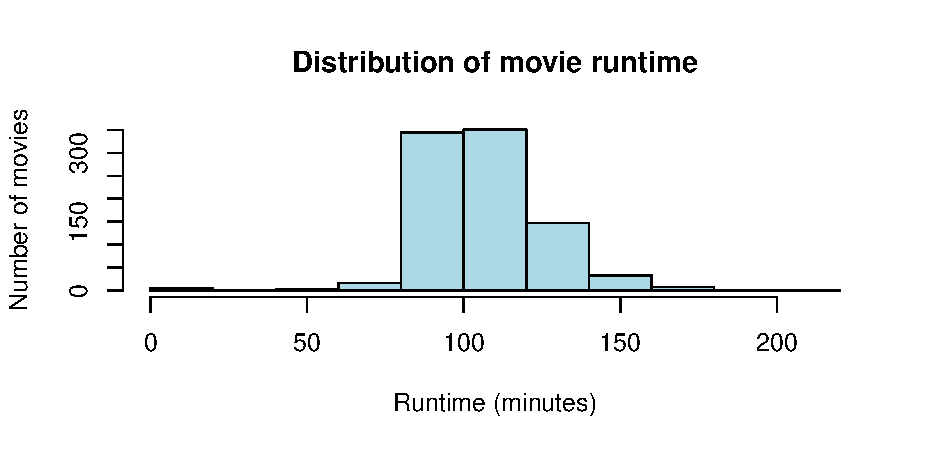
\includegraphics[keepaspectratio]{Untitled_files/Untitled_files/figure-latex/unnamed-chunk-19-1.pdf}}

\textbf{Your Answer:}

The chi-squared test in step a relies on the idea that runtime follows a
normal distribution in the population. To check this, we looked at a
histogram. There's a clear cluster of movies between 80 and 120 minutes,
and the center does look somewhat bell-shaped. But the right side
stretches out much further, and there are a few very short
runtimes---some are even zero. So, the distribution isn't clearly
normal. With this in mind, the normality assumption is shaky, and we
need to be cautious about any conclusions from step a.

\newpage

\subsection{3 Movie ratings and
profits}\label{movie-ratings-and-profits}

There is an argument going on in the movie studio. Bob claims that they
should make higher-quality movies, as this will bring in more profits.
Chantal disagrees. She tells Bob that mediocre movies bring the most
profits. You are asked to advise on who is right.

\subsubsection{Step a}\label{step-a-5}

Create a new variable called vote\_average\_rounded. Make sure this
variable is the same as vote\_average, but without any decimals (i.e., a
6.3 becomes a 6, a 8.7 an 8, etc.). Display a histogram of
vote\_average\_rounded. {[}2 points{]}

\begin{Shaded}
\begin{Highlighting}[]
\CommentTok{\# Remove decimals, following the examples in the question}
\NormalTok{movies}\SpecialCharTok{$}\NormalTok{vote\_average\_rounded }\OtherTok{\textless{}{-}} \FunctionTok{floor}\NormalTok{(movies}\SpecialCharTok{$}\NormalTok{vote\_average)}

\FunctionTok{hist}\NormalTok{(movies}\SpecialCharTok{$}\NormalTok{vote\_average\_rounded,}
     \AttributeTok{breaks =} \FunctionTok{seq}\NormalTok{(}\SpecialCharTok{{-}}\FloatTok{0.5}\NormalTok{, }\FloatTok{10.5}\NormalTok{, }\AttributeTok{by =} \DecValTok{1}\NormalTok{),}
     \AttributeTok{main =} \StringTok{"Distribution of movie ratings"}\NormalTok{,}
     \AttributeTok{xlab =} \StringTok{"Rating without decimals"}\NormalTok{,}
     \AttributeTok{ylab =} \StringTok{"Number of movies"}\NormalTok{,}
     \AttributeTok{col =} \StringTok{"lightblue"}\NormalTok{)}
\end{Highlighting}
\end{Shaded}

\pandocbounded{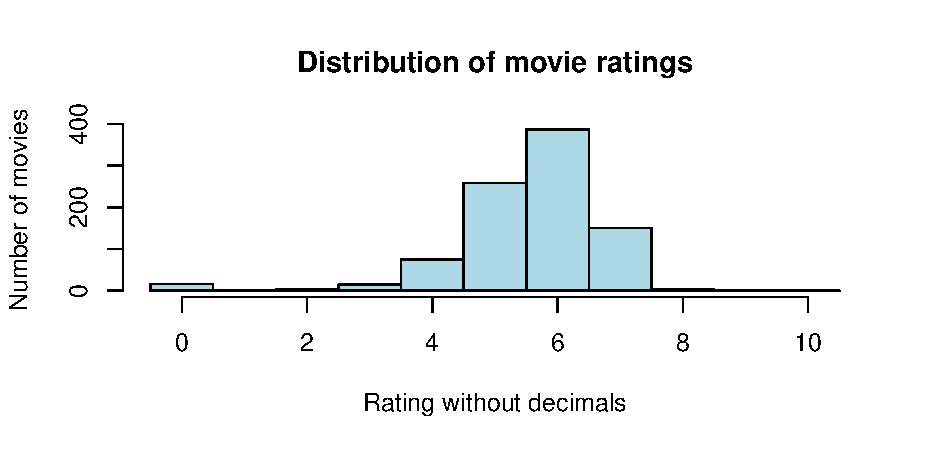
\includegraphics[keepaspectratio]{Untitled_files/Untitled_files/figure-latex/unnamed-chunk-20-1.pdf}}

\begin{Shaded}
\begin{Highlighting}[]

\FunctionTok{table}\NormalTok{(movies}\SpecialCharTok{$}\NormalTok{vote\_average\_rounded)}
\DocumentationTok{\#\# }
\DocumentationTok{\#\#   0   2   3   4   5   6   7   8   9 }
\DocumentationTok{\#\#  16   4  14  75 258 387 150   4   1}
\end{Highlighting}
\end{Shaded}

\textbf{Your Answer:}

We removed the decimals using floor(), so 6.3 becomes 6 and 8.7 becomes
8, as in the question. Most movies are in rating groups 5, 6 and 7.
Group 6 is the largest, with 387 movies. There are only 4 movies in
group 8 and 1 movie in group 9.

\subsubsection{Step b}\label{step-b-5}

Create a scatter plot with vote\_average\_rounded on the x axis and the
mean of profits within each category of vote\_average\_rounded on the
y-axis. Make sure it has an appropriate title, and appropriate titles
and labels for the x- and y-axis. At which rating of movies are the
profits the highest? {[}3 points{]}

\begin{Shaded}
\begin{Highlighting}[]
\CommentTok{\# Calculate the mean profit for each rating group}
\CommentTok{\# Profits are already expressed in millions in week 2}
\NormalTok{profits\_by\_rating }\OtherTok{\textless{}{-}} \FunctionTok{aggregate}\NormalTok{(profits }\SpecialCharTok{\textasciitilde{}}\NormalTok{ vote\_average\_rounded,}
                               \AttributeTok{data =}\NormalTok{ movies, }\AttributeTok{FUN =}\NormalTok{ mean)}

\NormalTok{profits\_by\_rating}
\DocumentationTok{\#\#   vote\_average\_rounded     profits}
\DocumentationTok{\#\# 1                    0  {-}0.4679164}
\DocumentationTok{\#\# 2                    2   0.0000000}
\DocumentationTok{\#\# 3                    3  {-}6.3909355}
\DocumentationTok{\#\# 4                    4   7.1176854}
\DocumentationTok{\#\# 5                    5  32.9318060}
\DocumentationTok{\#\# 6                    6  66.8883377}
\DocumentationTok{\#\# 7                    7 107.5850569}
\DocumentationTok{\#\# 8                    8  51.4821905}
\DocumentationTok{\#\# 9                    9   0.0000000}

\FunctionTok{plot}\NormalTok{(profits\_by\_rating}\SpecialCharTok{$}\NormalTok{vote\_average\_rounded,}
\NormalTok{     profits\_by\_rating}\SpecialCharTok{$}\NormalTok{profits,}
     \AttributeTok{main =} \StringTok{"Average movie profits by rating"}\NormalTok{,}
     \AttributeTok{xlab =} \StringTok{"Rating without decimals"}\NormalTok{,}
     \AttributeTok{ylab =} \StringTok{"Mean profit (millions)"}\NormalTok{,}
     \AttributeTok{pch =} \DecValTok{19}\NormalTok{,}
     \AttributeTok{col =} \StringTok{"blue"}\NormalTok{)}
\end{Highlighting}
\end{Shaded}

\pandocbounded{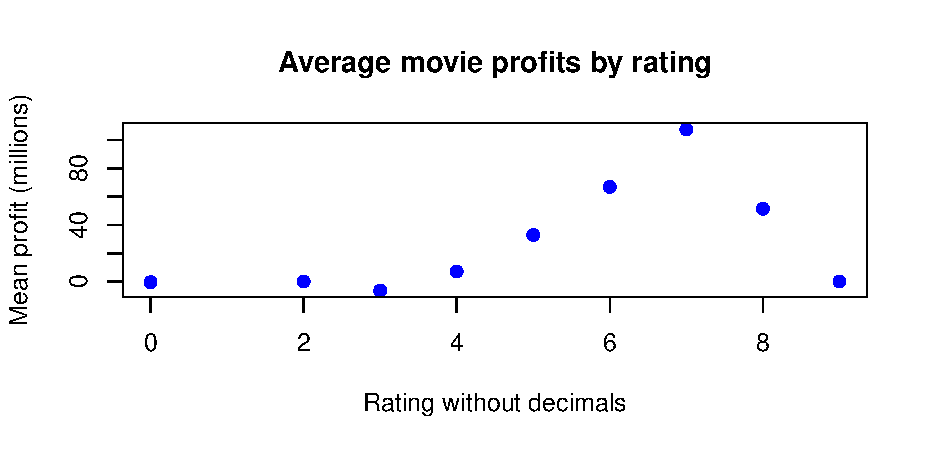
\includegraphics[keepaspectratio]{Untitled_files/Untitled_files/figure-latex/unnamed-chunk-21-1.pdf}}

\begin{Shaded}
\begin{Highlighting}[]

\NormalTok{profits\_by\_rating[}\FunctionTok{which.max}\NormalTok{(profits\_by\_rating}\SpecialCharTok{$}\NormalTok{profits), ]}
\DocumentationTok{\#\#   vote\_average\_rounded  profits}
\DocumentationTok{\#\# 7                    7 107.5851}
\end{Highlighting}
\end{Shaded}

\textbf{Your Answer:}

Rating group 7 has the highest mean profit, at approximately 107.59
million. This group contains movies with original ratings from 7.0 up to
(but not including) 8.0.

Mean profits generally increase as you move from the lower rating groups
to group 7. After that, profits drop off for groups 8 and 9. So, in this
given sample, the movies with the highest ratings don't actually bring
in the highest average (mean) profits.

\subsubsection{Step c}\label{step-c-3}

Recreate the scatter plot with year on the x axis and mean profits on
the y-axis, but now add bars around each point, indicating the 95\%
confidence interval. {[}3 points{]}

\begin{Shaded}
\begin{Highlighting}[]
\CommentTok{\# List the release years from lowest to highest}
\NormalTok{years }\OtherTok{\textless{}{-}} \FunctionTok{sort}\NormalTok{(}\FunctionTok{unique}\NormalTok{(movies}\SpecialCharTok{$}\NormalTok{release\_year))}

\NormalTok{mean\_profits\_year }\OtherTok{\textless{}{-}} \FunctionTok{numeric}\NormalTok{(}\FunctionTok{length}\NormalTok{(years))}
\NormalTok{lower\_profits\_year }\OtherTok{\textless{}{-}} \FunctionTok{numeric}\NormalTok{(}\FunctionTok{length}\NormalTok{(years))}
\NormalTok{upper\_profits\_year }\OtherTok{\textless{}{-}} \FunctionTok{numeric}\NormalTok{(}\FunctionTok{length}\NormalTok{(years))}

\CommentTok{\# Calculate the mean profit and 95\% confidence interval for each year}
\ControlFlowTok{for}\NormalTok{ (i }\ControlFlowTok{in} \DecValTok{1}\SpecialCharTok{:}\FunctionTok{length}\NormalTok{(years)) \{}
\NormalTok{  year\_profits }\OtherTok{\textless{}{-}}\NormalTok{ movies}\SpecialCharTok{$}\NormalTok{profits[movies}\SpecialCharTok{$}\NormalTok{release\_year }\SpecialCharTok{==}\NormalTok{ years[i]]}

\NormalTok{  mean\_profits\_year[i] }\OtherTok{\textless{}{-}} \FunctionTok{mean}\NormalTok{(year\_profits)}
\NormalTok{  standard\_error\_year }\OtherTok{\textless{}{-}} \FunctionTok{sd}\NormalTok{(year\_profits) }\SpecialCharTok{/} \FunctionTok{sqrt}\NormalTok{(}\FunctionTok{length}\NormalTok{(year\_profits))}

\NormalTok{  margin\_year }\OtherTok{\textless{}{-}} \FunctionTok{qt}\NormalTok{(}\FloatTok{0.975}\NormalTok{, }\AttributeTok{df =} \FunctionTok{length}\NormalTok{(year\_profits) }\SpecialCharTok{{-}} \DecValTok{1}\NormalTok{) }\SpecialCharTok{*}
\NormalTok{    standard\_error\_year}

\NormalTok{  lower\_profits\_year[i] }\OtherTok{\textless{}{-}}\NormalTok{ mean\_profits\_year[i] }\SpecialCharTok{{-}}\NormalTok{ margin\_year}
\NormalTok{  upper\_profits\_year[i] }\OtherTok{\textless{}{-}}\NormalTok{ mean\_profits\_year[i] }\SpecialCharTok{+}\NormalTok{ margin\_year}
\NormalTok{\}}

\FunctionTok{plot}\NormalTok{(years, mean\_profits\_year,}
     \AttributeTok{main =} \StringTok{"Average movie profits by release year"}\NormalTok{,}
     \AttributeTok{xlab =} \StringTok{"Release year"}\NormalTok{,}
     \AttributeTok{ylab =} \StringTok{"Mean profit (millions)"}\NormalTok{,}
     \AttributeTok{ylim =} \FunctionTok{range}\NormalTok{(lower\_profits\_year, upper\_profits\_year),}
     \AttributeTok{pch =} \DecValTok{19}\NormalTok{,}
     \AttributeTok{col =} \StringTok{"blue"}\NormalTok{)}

\CommentTok{\# Add the confidence interval bars}
\FunctionTok{arrows}\NormalTok{(}\AttributeTok{x0 =}\NormalTok{ years, }\AttributeTok{y0 =}\NormalTok{ lower\_profits\_year,}
       \AttributeTok{x1 =}\NormalTok{ years, }\AttributeTok{y1 =}\NormalTok{ upper\_profits\_year,}
       \AttributeTok{angle =} \DecValTok{90}\NormalTok{, }\AttributeTok{code =} \DecValTok{3}\NormalTok{, }\AttributeTok{length =} \FloatTok{0.05}\NormalTok{,}
       \AttributeTok{col =} \StringTok{"blue"}\NormalTok{)}
\end{Highlighting}
\end{Shaded}

\pandocbounded{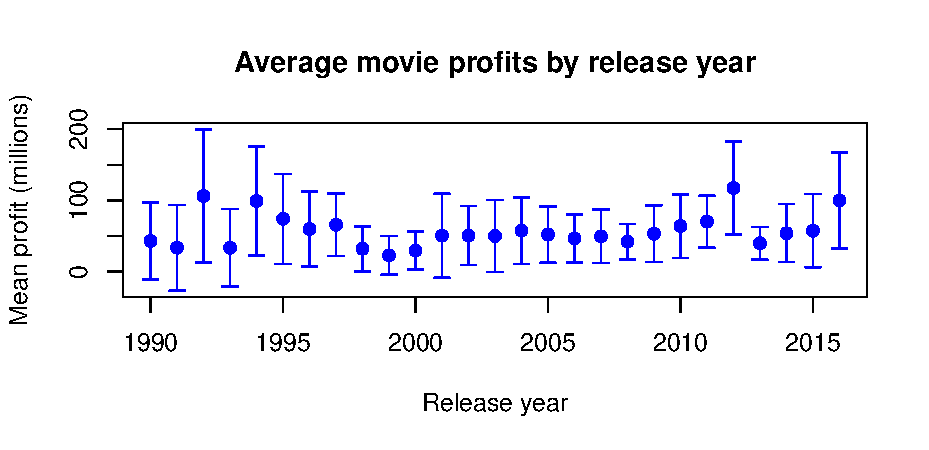
\includegraphics[keepaspectratio]{Untitled_files/Untitled_files/figure-latex/unnamed-chunk-22-1.pdf}}

\textbf{Your Answer:}

The plot shows the mean profit for each release year, with bars showing
its 95\% confidence interval. The highest mean profit is in 2012, at
approximately 117.49 million. Its confidence interval runs from 52.28 to
182.70 million.

Many intervals are wide, showing that the estimates are uncertain. Movie
profits vary a lot, and some years contain few movies. These t-intervals
are approximate because profits are strongly skewed, especially for
years with small samples. This plot compares release years, as requested
in the question.

\subsubsection{Step d}\label{step-d-2}

Write an advice to settle the argument between Bob and Chantal. {[}4
points{]}

\textbf{Your Answer:}

Our results do not clearly show that either Bob or Chantal is right.
Rating group 7 has the highest average profit, at about 107.59 million.
Groups 5 and 6 have lower average profits of 32.93 million and 66.89
million. If we consider groups 5 and 6 to be mediocre, this does not
support Chantal's claim in this sample.

However, higher ratings do not always go together with higher profits.
Group 8 has an average profit of 51.48 million. Group 9 has a calculated
average profit of zero, based on the recorded revenue and budget. Both
values are zero for its only movie, so we cannot conclude that it
actually earned nothing. Groups 8 and 9 contain only 4 movies and 1
movie, so we cannot draw strong conclusions about these groups.

We advise the studio to make movies that audiences enjoy, but a higher
rating does not guarantee more profit. Budget, genre and marketing may
also matter. These results do not prove that better movies cause higher
profits. The confidence intervals in step c compare release years, so
they do not show whether differences between rating groups are
statistically significant.

\end{document}
